\documentclass[tikz,border=8pt]{standalone}
% Shared look for every TikZ diagram. Load with % Shared look for every TikZ diagram. Load with % Shared look for every TikZ diagram. Load with \input{../../tools/tikz-style.tex}
\usepackage[T1]{fontenc}
\usepackage{lmodern}
\renewcommand{\sfdefault}{lmr}  % diagrams use the same serif as the text
\usetikzlibrary{arrows.meta, positioning, shapes.geometric, calc, fit, backgrounds}
\definecolor{cblue}{HTML}{4C78A8}
\definecolor{corange}{HTML}{F58518}
\definecolor{cgreen}{HTML}{54A24B}
\definecolor{cred}{HTML}{E45756}
\definecolor{cpurple}{HTML}{B279A2}
\definecolor{cgrey}{HTML}{6B6B6B}
\tikzset{
  every picture/.style={font=\sffamily, line width=1.2pt},
  box/.style={draw=#1, fill=#1!12, rounded corners=4pt, align=center, inner sep=7pt, minimum height=1.1cm},
  box/.default=cgrey,
  arrow/.style={-{Stealth[length=3mm]}, draw=cgrey, line width=1.4pt},
  title/.style={font=\sffamily\bfseries\Large},
  note/.style={font=\sffamily\small, text=cgrey, align=center},
}
\AtBeginDocument{\hyphenpenalty=10000 \exhyphenpenalty=10000}

\usepackage[T1]{fontenc}
\usepackage{lmodern}
\renewcommand{\sfdefault}{lmr}  % diagrams use the same serif as the text
\usetikzlibrary{arrows.meta, positioning, shapes.geometric, calc, fit, backgrounds}
\definecolor{cblue}{HTML}{4C78A8}
\definecolor{corange}{HTML}{F58518}
\definecolor{cgreen}{HTML}{54A24B}
\definecolor{cred}{HTML}{E45756}
\definecolor{cpurple}{HTML}{B279A2}
\definecolor{cgrey}{HTML}{6B6B6B}
\tikzset{
  every picture/.style={font=\sffamily, line width=1.2pt},
  box/.style={draw=#1, fill=#1!12, rounded corners=4pt, align=center, inner sep=7pt, minimum height=1.1cm},
  box/.default=cgrey,
  arrow/.style={-{Stealth[length=3mm]}, draw=cgrey, line width=1.4pt},
  title/.style={font=\sffamily\bfseries\Large},
  note/.style={font=\sffamily\small, text=cgrey, align=center},
}
\AtBeginDocument{\hyphenpenalty=10000 \exhyphenpenalty=10000}

\usepackage[T1]{fontenc}
\usepackage{lmodern}
\renewcommand{\sfdefault}{lmr}  % diagrams use the same serif as the text
\usetikzlibrary{arrows.meta, positioning, shapes.geometric, calc, fit, backgrounds}
\definecolor{cblue}{HTML}{4C78A8}
\definecolor{corange}{HTML}{F58518}
\definecolor{cgreen}{HTML}{54A24B}
\definecolor{cred}{HTML}{E45756}
\definecolor{cpurple}{HTML}{B279A2}
\definecolor{cgrey}{HTML}{6B6B6B}
\tikzset{
  every picture/.style={font=\sffamily, line width=1.2pt},
  box/.style={draw=#1, fill=#1!12, rounded corners=4pt, align=center, inner sep=7pt, minimum height=1.1cm},
  box/.default=cgrey,
  arrow/.style={-{Stealth[length=3mm]}, draw=cgrey, line width=1.4pt},
  title/.style={font=\sffamily\bfseries\Large},
  note/.style={font=\sffamily\small, text=cgrey, align=center},
}
\AtBeginDocument{\hyphenpenalty=10000 \exhyphenpenalty=10000}

\begin{document}
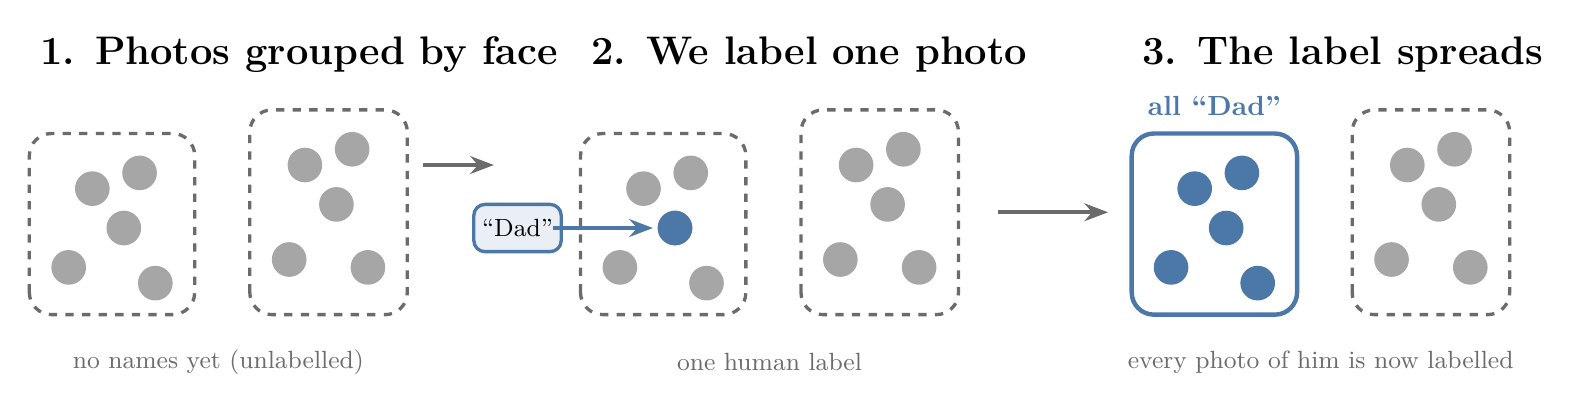
\begin{tikzpicture}
  \newcommand{\faces}[3]{% x offset, colour of group A, colour of group B
    \foreach \x/\y in {0.2/0.3, 0.9/0.8, 0.5/1.3, 1.3/0.1, 1.1/1.5} \fill[#2] (#1+\x,\y) circle (0.22);
    \foreach \x/\y in {3.0/0.4, 3.6/1.1, 3.2/1.6, 4.0/0.3, 3.8/1.8} \fill[#3] (#1+\x,\y) circle (0.22);
  }
  \node[title, anchor=west] at (-0.3,3.0) {1. Photos grouped by face};
  \faces{0}{cgrey!60}{cgrey!60}
  \draw[cgrey, dashed, rounded corners=8pt] (-0.3,-0.3) rectangle (1.8,2.0);
  \draw[cgrey, dashed, rounded corners=8pt] (2.5,-0.3) rectangle (4.5,2.3);
  \node[note] at (2.1,-0.9) {no names yet (unlabelled)};

  \node[title, anchor=west] at (6.7,3.0) {2. We label one photo};
  \faces{7}{cgrey!60}{cgrey!60}
  \fill[cblue] (7.9,0.8) circle (0.22);
  \draw[cgrey, dashed, rounded corners=8pt] (6.7,-0.3) rectangle (8.8,2.0);
  \draw[cgrey, dashed, rounded corners=8pt] (9.5,-0.3) rectangle (11.5,2.3);
  \node[box=cblue, font=\sffamily\small, inner sep=3pt, minimum height=0.6cm] at (5.9,0.8) {``Dad''};
  \draw[arrow, draw=cblue] (6.35,0.8) -- (7.62,0.8);
  \node[note] at (9.1,-0.9) {one human label};

  \node[title, anchor=west] at (13.7,3.0) {3. The label spreads};
  \faces{14}{cblue}{cgrey!60}
  \draw[cblue, rounded corners=8pt, line width=1.6pt] (13.7,-0.3) rectangle (15.8,2.0);
  \node[cblue, font=\sffamily\bfseries] at (14.75,2.35) {all ``Dad''};
  \draw[cgrey, dashed, rounded corners=8pt] (16.5,-0.3) rectangle (18.5,2.3);
  \node[note] at (16.1,-0.9) {every photo of him is now labelled};
  \draw[arrow] (4.7,1.6) -- (5.6,1.6);
  \draw[arrow] (12.0,1.0) -- (13.4,1.0);
\end{tikzpicture}
\end{document}
